% Options for packages loaded elsewhere
\PassOptionsToPackage{unicode}{hyperref}
\PassOptionsToPackage{hyphens}{url}
%
\documentclass[
]{book}
\usepackage{lmodern}
\usepackage{amssymb,amsmath}
\usepackage{ifxetex,ifluatex}
\ifnum 0\ifxetex 1\fi\ifluatex 1\fi=0 % if pdftex
  \usepackage[T1]{fontenc}
  \usepackage[utf8]{inputenc}
  \usepackage{textcomp} % provide euro and other symbols
\else % if luatex or xetex
  \usepackage{unicode-math}
  \defaultfontfeatures{Scale=MatchLowercase}
  \defaultfontfeatures[\rmfamily]{Ligatures=TeX,Scale=1}
\fi
% Use upquote if available, for straight quotes in verbatim environments
\IfFileExists{upquote.sty}{\usepackage{upquote}}{}
\IfFileExists{microtype.sty}{% use microtype if available
  \usepackage[]{microtype}
  \UseMicrotypeSet[protrusion]{basicmath} % disable protrusion for tt fonts
}{}
\makeatletter
\@ifundefined{KOMAClassName}{% if non-KOMA class
  \IfFileExists{parskip.sty}{%
    \usepackage{parskip}
  }{% else
    \setlength{\parindent}{0pt}
    \setlength{\parskip}{6pt plus 2pt minus 1pt}}
}{% if KOMA class
  \KOMAoptions{parskip=half}}
\makeatother
\usepackage{xcolor}
\IfFileExists{xurl.sty}{\usepackage{xurl}}{} % add URL line breaks if available
\IfFileExists{bookmark.sty}{\usepackage{bookmark}}{\usepackage{hyperref}}
\hypersetup{
  pdftitle={Gambling Statistics},
  pdfauthor={Dan Rogers},
  hidelinks,
  pdfcreator={LaTeX via pandoc}}
\urlstyle{same} % disable monospaced font for URLs
\usepackage{longtable,booktabs}
% Correct order of tables after \paragraph or \subparagraph
\usepackage{etoolbox}
\makeatletter
\patchcmd\longtable{\par}{\if@noskipsec\mbox{}\fi\par}{}{}
\makeatother
% Allow footnotes in longtable head/foot
\IfFileExists{footnotehyper.sty}{\usepackage{footnotehyper}}{\usepackage{footnote}}
\makesavenoteenv{longtable}
\usepackage{graphicx,grffile}
\makeatletter
\def\maxwidth{\ifdim\Gin@nat@width>\linewidth\linewidth\else\Gin@nat@width\fi}
\def\maxheight{\ifdim\Gin@nat@height>\textheight\textheight\else\Gin@nat@height\fi}
\makeatother
% Scale images if necessary, so that they will not overflow the page
% margins by default, and it is still possible to overwrite the defaults
% using explicit options in \includegraphics[width, height, ...]{}
\setkeys{Gin}{width=\maxwidth,height=\maxheight,keepaspectratio}
% Set default figure placement to htbp
\makeatletter
\def\fps@figure{htbp}
\makeatother
\setlength{\emergencystretch}{3em} % prevent overfull lines
\providecommand{\tightlist}{%
  \setlength{\itemsep}{0pt}\setlength{\parskip}{0pt}}
\setcounter{secnumdepth}{5}
\usepackage{booktabs}
\usepackage{amsthm}
\makeatletter
\def\thm@space@setup{%
  \thm@preskip=8pt plus 2pt minus 4pt
  \thm@postskip=\thm@preskip
}
\makeatother
\usepackage[]{natbib}
\bibliographystyle{plainnat}

\title{Gambling Statistics}
\author{Dan Rogers}
\date{2020-10-17}

\begin{document}
\maketitle

{
\setcounter{tocdepth}{1}
\tableofcontents
}
\hypertarget{introduction}{%
\chapter*{Introduction}\label{introduction}}
\addcontentsline{toc}{chapter}{Introduction}

I remember being about 16 years old, spending a few weeks each summer at Devil's Lake with my grandparents. One of the fun things we would do is get the felt casino cover for the table out. It had a Blackjack table on one side and Craps on the other. Grandpa would be the house, calling out our bets, informing us of bad bets, and paying out the winner.

During one of those summers, I had just learned about calculating sums for inifinite series. I remember trying to calculate the odds on craps, and realizing it was an infinite series that could be summed just like we had learned in class. This was really quite amazing. While it was widely believed we would never actually use the math we were learning in class, here was a great example of how it can be used in real life

That example of using math to calculate the expected returns in craps stands out in my mind as something that really drove my interest in gambling and applying statistics to different games. It wasn't too long after that I was also building computer simulations for games like Blackjack and Poker, trying to re-create basic strategy and the different statistical tables I had seen for Texas Hold 'Em.

Now I'll be the first to admit: this is well-trodden ground that doesn't require any new work or discovery by me. The \href{https://wizardofodds.com/}{Wizard of Odds} has already calculated statistics and expected returns for pretty much any game you can imagine. There really isn't any value in me going through and calculating them all myself\ldots{} except that I like it. I think it's fun, and I've decided that is reason enough.

I intend to put my notes here as I accumulate them, adding a chapter for each game or subject. There's even a chance that this could turn into a good reference for statistics applied to gambling games. I intend to start with the most basic games and build up to the more complex. So maybe there is some value in arranging the content in this way and emphasizing the math that gets you to the answer rather than just the result. But really, when it comes down to it, I just find this a fun way to spend time, and that is all that matters.

\hypertarget{flipping-a-coin}{%
\chapter{Flipping a Coin (and Basic Probabilities)}\label{flipping-a-coin}}

\begin{figure}
\centering
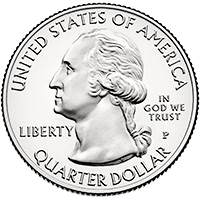
\includegraphics{images/quarter.png}
\caption{U.S. Quarter}
\end{figure}

The simplest game of chance I can imagine is flipping a coin. A fair coin will have a 50\% chance of coming up heads and 50\% chance of coming up tails. A fair bet is one that pays even money. That means that if you bet \$1 on a particular outcome (heads or tails), you win \$1 if you're right and lose \$1 if you're wrong. In gambling terms the \href{https://en.wikipedia.org/wiki/Odds}{``odds''} are 1-to-1, meaning there is an equal probability of each outcome, and a fair bet will pay 1-to-1, meaning that the dollar you bet is matched with 1 dollar you win.

The expected value of such a wager is calculated as:

\[ Expected Value = Pr(win) * (\$1) + Pr(lose) * (-\$1) = 0.5 * (\$1) + 0.5 * (-\$1) = \$0 \]

This is the basic means of calculating any expectation in statistics. First, you find the probabilities or each event. Next, you multiply each probability by the expected return in each scenario. And then you add those all together. The difficult part is usually finding the probabilities or each outcome, especially in games that involve player's making choices where you also must work to find the optimal choice in any scenario.

\hypertarget{roulette}{%
\chapter{Roulette}\label{roulette}}

\begin{figure}
\centering
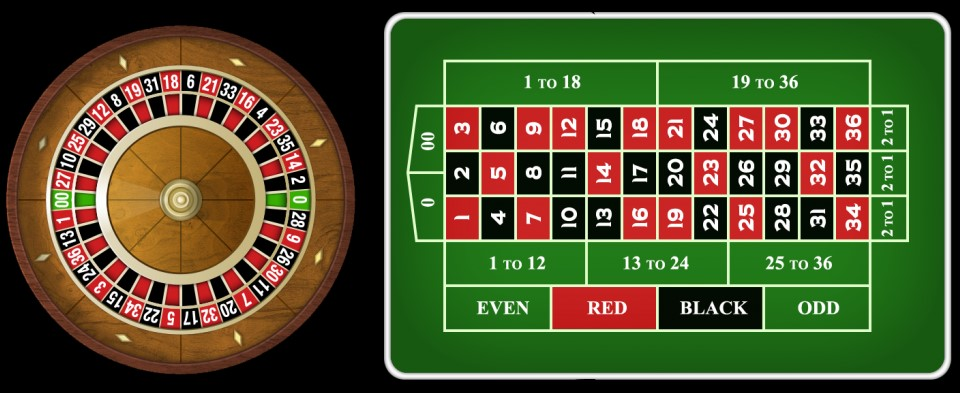
\includegraphics{images/roulette.jpg}
\caption{Roulette Table}
\end{figure}

Roulette is a fun and simple game where a large wheel is spun and then a ball is dropped into the wheel. Players bet on where the ball will land. The main numbers range from 1 to 36 and are divided into half red and half black. There is also an additional number: zero that is neither red nor black (nor is it even or odd). In most games, you will find zero (0) and double zero (00). The presence of these numbers is what gives the house its edge in the game.

There are a variety of bets that can be made in Roulette:

\begin{itemize}
\tightlist
\item
  Red or black, paying 1-to-1
\item
  Even or odd, paying 1-to-1
\item
  Any single number (``Straight Up''), paying 35-to-1
\item
  Two adjacent numbers (``Split''), paying 17 to 1
\item
  Three numbers in a row (``Street''), paying 11 to 1
\item
  Four adjoining numbers (``Corner''), paying 8 to 1
\item
  Twelve numbers, either sequential (``Dozen'') or in a ``Column'', paying 2 to 1
\item
  1-18 or 19-36, paying 1-to-1
\end{itemize}

Interestingly, the expected return on all of these bets is exactly the same. To show why this is true, let's calculate a few. First, we'll calculate my favorite bet: red or black, paying even money.

\[ Expected Value = \frac{18}{38} * (\$1) + \frac{20}{38} * (-\$1) = -\frac{2}{38} = -0.05263158 \]

Notice that this bet is almost like flipping a coin (\ref{flipping-a-coin}). In fact, if the zeroes were not on the board and we only had 36 numbers, it would be identical. However, the presence of the zeroes means that we have 38 outcomes, not 36, and the 2 new outcomes that are introduced by the presence of the zero are losses for us. This turns the expected return slightly negative, giving the house a 5.26\% edge. However much money we place on this bet, we should expect to lose an average of 5.26\% with each spin of the wheel.

Let's calculate another one. Obviously, the even or odd bet will be the same. So let's do a straight up bet on a single number. The expected return in this case is:

\[ Expected Value = \frac{1}{38} * (\$35) + \frac{37}{38} * (-\$1) = -\frac{2}{38} = -0.05263158 \]

As suggested, this is the the same house edge as the red/black or even/odd bet. Knowing that the payout on any bet is equal to the true odds in the absence of the zeroes, we can see that this will always come out the same way. Just to demonstrate this, here are the expected values for bets place on 4 and 12 numbers:

\[ Expected Value = \frac{4}{38} * (\$8) + \frac{34}{38} * (-\$1) = -\frac{2}{38} = -0.05263158 \]

\[ Expected Value = \frac{12}{38} * (\$2) + \frac{26}{38} * (-\$1) = -\frac{2}{38} = -0.05263158 \]

So far we have analyzed ``American'' roulette, which has both zero and double zero. ``European'' roulette instead only has 1 zero. Intuitively, we know that this will improve our odds. Specifically, we find that a single number bet now has the expected value:

\[ Expected Value = \frac{1}{37} * (\$1) + \frac{36}{37} * (-\$1) = -\frac{1}{37} = 0.02702703 \]

The house edge has been cut almost in half, from 5.26\% to 2.70\%. As with ``American'' roulette, all of the other bets will have this same expected value and house edge. Obviously, it is advantageous to players to play at ``European'' style tables whenever possible.

\hypertarget{craps}{%
\chapter{Craps}\label{craps}}

\hypertarget{baccarat}{%
\chapter{Baccarat}\label{baccarat}}

\hypertarget{overview}{%
\section{Overview}\label{overview}}

Baccarat is often mentioned as a classy game (James Bond plays it in movies) and one where billionaire ``whales'' can win (or lose) millions of dollars in a single night. It also has one of the smallest house edges in the casino. According to \href{https://en.wikipedia.org/wiki/Baccarat_(card_game)}{Wikipedia} it is played with 6-8 decks and follows a somewhat complicated set of rules for dealing cards to a ``player'' and a ``banker''. Observers of the game bet on whether the ``player'' or ``banker'' will win. They also can bet on a ``tie''.

According to Wikipedia, the typical payouts and house advantages for these scenarios (with a 8-deck shoe) are below:

\begin{longtable}[]{@{}lrr@{}}
\toprule
Outcome & Payout & House Edge\tabularnewline
\midrule
\endhead
Banker Wins & 19-to-20 & 1.06\%\tabularnewline
Player Wins & 1-to-1 & 1.24\%\tabularnewline
Tie & 8-to-1 & 14.4\%\tabularnewline
\bottomrule
\end{longtable}

\hypertarget{simulation}{%
\section{Simulation}\label{simulation}}

I wrote a Baccarat simulator in Java to confirm these numbers. The simulator played 1 billion hands of Baccarat following the classic ``Punto Banco'' rules as described on Wikipedia. This took about 4 minutes to run. The results were:

\begin{longtable}[]{@{}lrr@{}}
\toprule
Winner & Occurrences & Percentage\tabularnewline
\midrule
\endhead
Banker Wins & 458,618,223 & 45.8618223\%\tabularnewline
Player Wins & 446,309,890 & 44.6309890\%\tabularnewline
Tie & 95,071,887 & 9.5071887\%\tabularnewline
Total & 1,000,000,000 & 100.0000000\%\tabularnewline
\bottomrule
\end{longtable}

To calculate the expected return and house advantage we need to include the payouts that result from the bets for each scenario. This is shown in the table below:

\begin{longtable}[]{@{}lrrr@{}}
\toprule
Outcome & Return(B) & Return(P) & Return(T)\tabularnewline
\midrule
\endhead
Banker Wins & 1.95 & 0 & 0\tabularnewline
Player Wins & 0 & 2.00 & 0\tabularnewline
Tie & 1.00 & 1.00 & 9.00\tabularnewline
\bottomrule
\end{longtable}

Return(B) indicates the money you receive in each scenario if you bet on the banker winning. Similarly, Return(P) and Return(T) represent bets placed on the player and a tie.

When multiplying these returns by the probability of each scenario, the expected returns and house advantages for each bet are:

\begin{longtable}[]{@{}lrr@{}}
\toprule
Bet & Expected Return & House Advantage\tabularnewline
\midrule
\endhead
Banker & 98.94\% & 1.06\%\tabularnewline
Player & 98.77\% & 1.23\%\tabularnewline
Tie & 85.56\% & 14.44\%\tabularnewline
\bottomrule
\end{longtable}

These match the results from Wikipedia to within +/- .01\%.

If we wanted to get fancy, we could calculate confidence intervals around our estimates. To do this, we make use of the fact that the Bernoulli distribution has a variance of ``p(1-p)''. This means that when calculating p as an average of N observations we would expect a standard deviation of ``p(1-p) / sqrt(N)'' around our estimate of the mean. This allows us to create the following confidence intervals around our probabilities:

\begin{longtable}[]{@{}lrrrr@{}}
\toprule
Outcome & Estimate & Stdev(Estimate) & Min(Estimate) & Max(Estimate)\tabularnewline
\midrule
\endhead
Banker Wins & 45.8618223\% & 0.00157571\% & 45.8570952\% & 45.8665494\%\tabularnewline
Player Wins & 44.6309890\% & 0.001572\% & 44.6262730\% & 44.635705\%\tabularnewline
Tie & 9.5071887\% & 0.000927541\% & 9.5044061\% & 9.5099713\%\tabularnewline
\bottomrule
\end{longtable}

The Min and Max values of the estimate are calculated using 3 standard deviations. This means that we have a 99\% chance of the true probability being somewhere between these two values.

We can use these min and max estimates to calculate the payouts. This time we get:

\begin{longtable}[]{@{}lrr@{}}
\toprule
Bet & Expected Return & House Advantage\tabularnewline
\midrule
\endhead
Banker & 98.93 - 98.95\% & 1.05 - 1.07\%\tabularnewline
Player & 98.76 - 98.78\% & 1.22 - 1.24\%\tabularnewline
Tie & 85.54 - 85.59\% & 14.41 - 14.46\%\tabularnewline
\bottomrule
\end{longtable}

1 billion hands are needed in order to get confidence intervals this small. It is pleasing to see that the exact values from Wikipedia fall into our confidence ranges.

\hypertarget{card-counting}{%
\section{Card Counting}\label{card-counting}}

Since Baccarat is played from a 6- or 8-deck shoe, you might naturally think there is an opportunity to count cards. The article below provides a great summary of several experts on this subject, each of them indicating that card counting is not practical in this game:

\begin{itemize}
\tightlist
\item
  \url{https://www.888casino.com/blog/baccarat-tips/card-counting-in-baccarat}
\end{itemize}

The reason for this is that - unlike Blackjack - there are not cards that clearly favor the player or the banker. There are also no choices made in the game (except for your bet size), meaning that you can't use your knowledge of the deck to play the cards differently.

Ed Thorp does provide a card-counting strategy that can yield an advantage to bets made on the player in rare scenarios. A positive advantage of 0.329\% occurs every 1,786 hands, which is far too rare to use to your advantage. John May (a baccarat author) developed a counting strategy for betting on a tie that he claims yields a 62\% advantage in certain rare scenarios. However, these rare scenarios occur approximately once every 10,000 hands - again making it too rare to be useful. If a player played Baccarat 40 hours a week, this scenario would occur only once every three weeks.

\end{document}
